In this section, we show the optimization details done through this work. We discuss the statistics of the new database and the schema changes. Moreover, other optimization techniques related to query, indexes and memory are discussed, as well.

\subsection{New Database Statistics}
In this subsection, we show the new database statistics after optimization. The record count is extracted from the database filled with $100000$ records per table. Other filling sizes are considered through the analysis like $10000$ and $1000000$. \\

\begin{tabular}{||c | c | c | c | c||} 
 \hline
 Table Name & Row Count & Main Key & Indexes & FK  \\ [0.5ex] 
 \hline\hline
 Disaster & 100000 & YES & 4 & 2 \\ 
 \hline\hline
 Causes & 100000 & YES & 1 & 1 \\ 
 \hline\hline
 Precautions & 100000 & YES & 1 & 1 \\ 
 \hline\hline
 Incident & 100000 & YES & 4 & 3 \\ 
 \hline\hline
 Descriptions & 100000 & YES & 1 & 1 \\ 
 \hline\hline
 Casualty & 25000 & YES & 1 & 0 \\ 
 \hline
 Government\_Representative & 25000 & YES & 1 & 0 \\
 \hline
 Govn\_Rep\_Credentials & 25000 & YES & 1 & 1 \\
 \hline
 Citizen & 25000 & YES & 1 & 0 \\
 \hline
 Citizen\_Credentials & 25000 & YES & 1 & 1 \\
 \hline
 Criminal & 25000 & YES & 1 & 0 \\
 \hline
 Report & 100000 & YES & 5 & 4 \\
 \hline
 Report\_Content & 100000 & YES & 1 & 1 \\
 \hline
 Casualty\_Incident & 100000 & YES \emph{(Composite)} & 3 & 2 \\ [1ex] 
 \hline
\end{tabular} \\

\begin{tabular}{||c | c | c||} 
 \hline
 Table Name & Identity Column & Max Row Size (Bytes) \\ [0.5ex] 
 \hline\hline
 Disaster & YES & 52 \\ 
 \hline
 Causes & YES & 65538 \\ 
 \hline
 Precautions & YES & 65538 \\ 
 \hline
 Incident & YES & 120 \\ 
 \hline
 Descriptions & YES & 65538 \\ 
 \hline
 Casualty & YES & 105 \\ 
 \hline
 Government\_Representative & YES & 116 \\ 
 \hline
 Govn\_Rep\_Credentials & YES & 103 \\ 
 \hline
 Citizen & YES & 116 \\ 
 \hline
 Citizen\_Credentials & YES & 103 \\ 
 \hline
 Criminal & YES & 106 \\ 
 \hline
 Report & YES & 23 \\ 
 \hline
 Report\_Content & YES & 65538 \\ 
 \hline
 Casualty\_Incident & NO & 6 \\ [1ex] 
 \hline
\end{tabular}

\subsection{Schema Optimization}
The following database schema shows the optimizations over the old schema. The schema optimizations can be summarized as follows :
\begin{enumerate}
    \item \textbf{Denormalization} of \emph{Person} table with all persons types. This is mainly because no duplicates between persons types. For example, no person can be a casualty and a criminal at the same time. So, in order to avoid redundant joins, the \emph{Person} relation is merged into the four child relations.
    \item \textbf{Normalization} \emph{(Vertical Partitioning)} of variable-size data. The access of fixed-size records is faster than that of variable-size data, as the \emph{DBMS} don't require to pre-calculate the record size. That's why, the variable-size data like \emph{text}, \emph{usernames} and \emph{passwords} are separated into separate relations. One more reason for doing so is that the data in these fields aren't accessed frequently, so they better be separate from other frequently-accessed data.
    \item \textbf{Minimization} of the data types based on semantic and statistical \emph{heuristics}. The data types of different fields are reduced to the minimum possible size, in order to ease their read and write to the disk. For example, all \emph{primary keys} are reduced to \texttt{MEDIUMINT}, because the table size is at most $1000000$. Moreover, Some fields that are just limited to range from $1$ to $10$ are reduced to $4$ bits instead of \texttt{INT}.
    \item \textbf{Conversion} of variable-size data to fixed-size data. As the fixed-size record are faster to access and transfer, so each \emph{VarChar} is converted into \emph{Char}. This, however, can increase the storage space, as \emph{Char} allocates the target bytes whatever they are all used or not.
    \item \textbf{Usage} of \texttt{NOT NULL}, whenever possible. If the field isn't marked as \texttt{NOT NULL}, it allocates extra bits to check whether the field is \emph{NULL} or not.
\end{enumerate}
\begin{figure}[H]
    \centering
    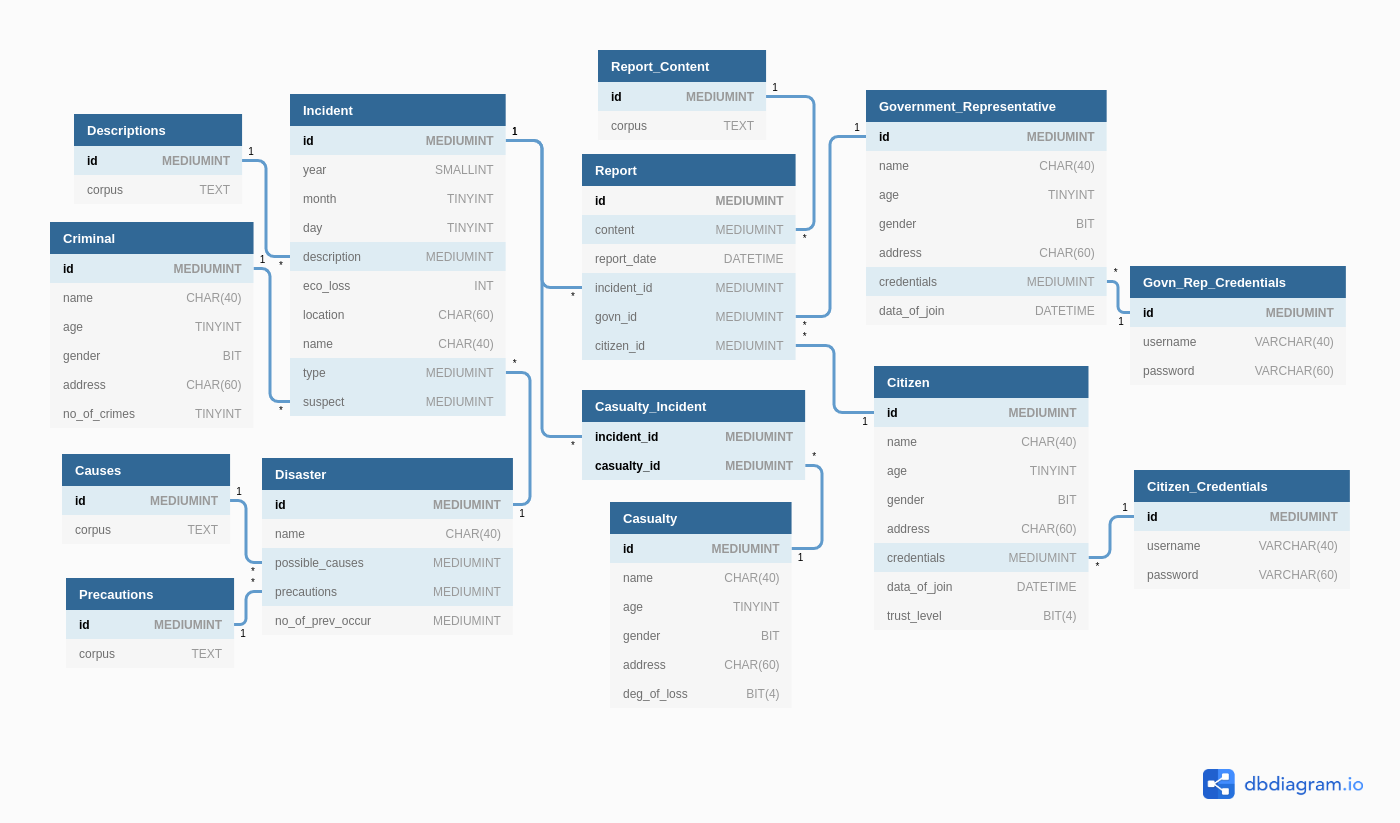
\includegraphics[width=\textwidth]{images/stats/optimized-schema.png}
    \caption{New Optimized Database Schema.}
    \label{fig:db-schema}
\end{figure}

\subsection{Memory Optimization}

\subsection{Index Tuning}

\subsection{Query Optimization}
\subsubsection{Query 1}
\subsubsection{Query 2}
\subsubsection{Query 3}
\subsubsection{Query 4}
\subsubsection{Query 5}
